\subsection{Motivation and overview}
\label{intro:overview}
The human gut holds a dense bacterial community alongside a large population of the viruses that infect it,
most of them bacteriophages \citep{shkoporov2019}. Infection requires a match between molecular structures on
both partners, so a phage generally infects only a narrow range of hosts, and in removing some bacteria and
not others it shapes the community. Shifts in that composition have been associated with colorectal cancer,
inflammatory bowel disease and graft-versus-host disease \citep{wirbel2019,lloydprice2019,peled2020}. Which
phage infects which bacterium is therefore worth knowing, and is rarely observed directly.

Two proxies are available from sequencing data, and they are of different kinds. A CRISPR spacer is a fragment of viral DNA
stored in the bacterial genome, so a spacer matching a viral genome shows that the bacterium's lineage was
infected by that virus at some point in the past; the match itself is found computationally
\citep{zhang2021spacepharer}. A co-abundance network, on the other hand, is estimated statistically: a
graphical lasso over abundances measured across samples marks pairs whose abundances covary once every other
organism is held fixed \citep{friedman2008,liu2010}.

Computational host prediction is an established problem, but existing approaches build their features from
curated references and assign a host taxon to a phage \citep{edwards2016,coutinho2021,roux2023,nie2024}. This
thesis describes organisms only by protein clusters formed \emph{de novo} within each cohort, without
functional annotation, and predicts both proxies on the identical set of genus--vOTU pairs in three cohorts.
Since the two targets are meant to describe one phenomenon, it also asks whether a single latent
representation can serve both.


\subsection{Research questions and outline}
\label{intro:questions}
The thesis addresses three questions.

\begin{enumerate}
  \item Can CRISPR linkage between a bacterial genus and a vOTU be predicted from an annotation-free
        protein-cluster representation of the two organisms?
  \item Can a co-abundance edge between the same pair be predicted from the same representation?
  \item Does a latent representation trained on both targets serve either better than one trained on a single
        target?
\end{enumerate}

The contribution is a controlled comparison: both proxies are predicted from identical features, on identical
folds, over the identical set of pairs, in three independent cohorts, so any difference between them is a
difference between the targets and not between the data or the models.

Figure~\ref{fig:pipeline-overview} summarises that setup. Each bacterial genus and each vOTU is described by its
own annotation-free protein-cluster profile; the two profiles are combined into a single pair representation,
and one model maps that representation to both targets.

\begin{figure}[htbp]
  \centering
  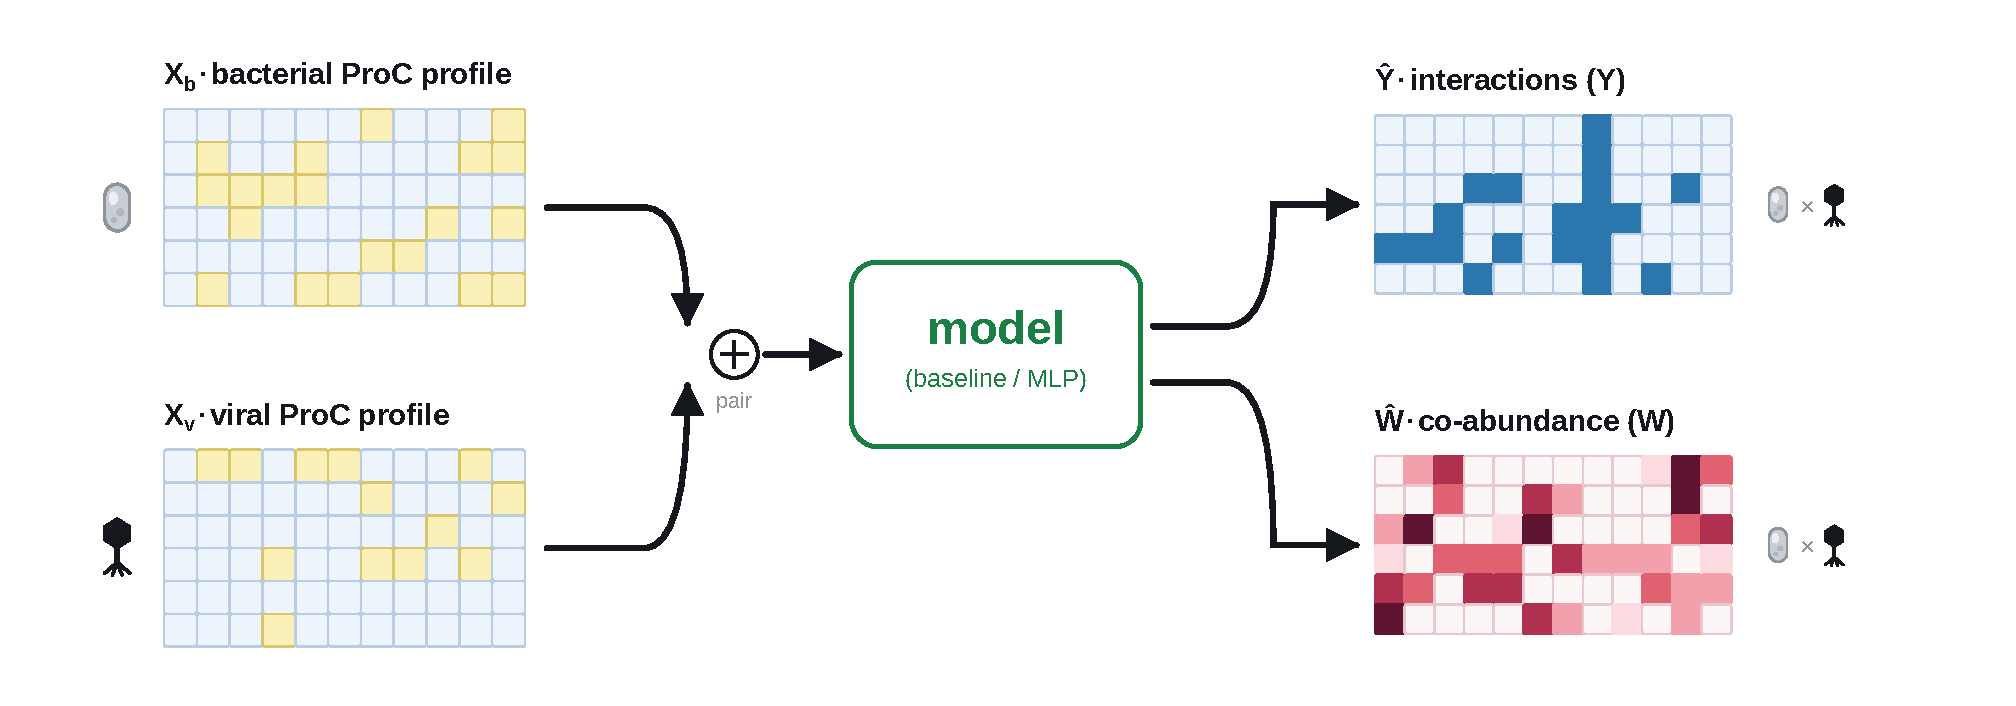
\includegraphics[width=\textwidth]{figures/fig_pipeline_overview.pdf}
  \caption{Overview of the prediction setup. A bacterial genus and a vOTU are each described by an
  annotation-free protein-cluster (ProC) profile, $X_b$ and $X_v$. The two profiles are combined into one
  pair representation, which a single model maps to both targets: CRISPR linkage $\hat{Y}$ and the glasso
  co-abundance edge $\hat{W}$. Both targets are predicted from the identical representation, on identical
  folds, over the identical set of genus--vOTU pairs. This figure was created by Claude Opus 5 (Anthropic).}
  \label{fig:pipeline-overview}
\end{figure}

